% ============================================================
% ch08：规模复现：ResNet-18 / CIFAR-100（对应论文 §5.7 "At scale"）
% 读者已读 tutorial/（EoS 入门）；本章讲论文增量。
% ============================================================

\section{规模复现：ResNet-18/CIFAR-100}\label{sec:ch08}

\begin{keybox}{本章速览}
\begin{itemize}
  \item MLP 上的三向对比（SGD / 秩-1 plant / SAM）搬上标准 torchvision
        ResNet-18（11.2M 参数，约为 MLP 的 $160\times$）+ CIFAR-100，$n=5$
        种子、ARPACK + 确定性 CUDA 协议：晚期 $\lmax$ 为 SGD
        $29.21\pm1.90$、rank-1 plant $28.83\pm1.67$、SAM $22.63\pm1.73$。
  \item 诚实读法是\emph{双结局}：SAM 的上置信界（$24.36$）不与
        SGD/rank-1 的下置信界（$27.31/27.16$）重叠，但 SGD 与 rank-1
        之间统计不可分——是 $\{\text{SGD}\approx\text{rank-1}\}$ 与 SAM
        的两方分裂，不是三向分裂。
  \item 一次方法论弯路：原 plant 的幂迭代感知\emph{伪收敛}把真实
        $\lmax\approx36$ 读成 $\approx19$（$+45\%$ 低估），一度被误读为
        “批尖锐度在 $2/\eta$”——\emph{proxy 坏了，不是体制坏了}。
  \item 换上 ARPACK 感知的 true-$\lmax$ plant 后，执行器确以全力开火
        （除数中位 $1.86$、每步阻尼因子 $\approx0.44$），$\lmax$ 仍与
        SGD 重叠：规模版的\emph{有动作仍被钉住}。
  \item 12000 步 + 标准增强的长日程保序（SAM $18.1 <$ SGD $21.9\approx$
        rank-1 $22.8$），且 SAM 精度最好（$0.68$ vs $0.66$）；ResNet-18
        上的 rank-$k$ 是 null 结果，排序结论（任何 $k$ 无下逃逸、唯
        SAM）在真实 CNN 上成立。
\end{itemize}
\end{keybox}

\textbf{本章在论文中的位置。}论文的控制实验（秩-1 阻尼、rank-$k$
扫描、X-SAM 消融、多尖锐景观测试）都发生在全批 GD 的小 MLP 上——这是
EoS 现象最干净的体制，但也是审稿人最容易质疑的地方：\emph{“控制实验都
源自 MLP，结论会不会是 MLP 特异的？”}论文 \S5.7（"At scale"）就是对这个
关切的正面回应：把三向对比（SGD、秩-1 plant、SAM）原样搬到标准
torchvision ResNet-18（11.2M 参数，约为 MLP 的 $160\times$）上，在
CIFAR-100 训练，$n=5$ 种子，并把测量协议升级为确定性 CUDA + ARPACK 直测。
本章按论文顺序讲四件事：三向对比的诚实读法（\S\ref{sec:ch08-threeway}）、
感知伪收敛的方法论插曲与 true-$\lmax$ plant 的“有动作仍被钉住”
（\S\ref{sec:ch08-falseconv}--\S\ref{sec:ch08-pinned}）、更长日程的外部效度
（external validity，结论超出当前实验设置仍然成立的能力；\S\ref{sec:ch08-long}）、以及 rank-$k$ 与“为何 SAM 能而 rank-1
不能”（\S\ref{sec:ch08-rankk}--\S\ref{sec:ch08-why}）。理论一侧的对应
形式化在第~\ref{sec:ch09}~章。

\subsection{先校准阈值：动量下边界是 $2(1+\mu)/\eta=38$，不是 $2/\eta=20$}\label{sec:ch08-threeway}

读者从本解读第 3 章已经知道：$2/\eta$ 定律是\emph{全批 GD} 的极限；在重球
动量（heavy-ball）下，线性稳定性边界移到 $2(1+\mu)/\eta$。ResNet-18 实验
用 $\mu=0.9$（由两边界 $38$ 与 $20$ 可读出 $\eta=0.1$），所以起作用的
边界是 $2(1+\mu)/\eta=38$，而 GD 边界 $2/\eta=20$ 只是参照线。这一步校准
很重要：如果把 20 当作期望钉住值，会误读所有绝对数字。

\textbf{判读口径提醒。}下文``逐种子排序不一致''指同一种子下两臂谁高
谁低在不同种子间来回翻转、无稳定次序——它是``统计不可分''的直观旁证
（判读规则见第~\ref{sec:ch03-stats}~节）。另注意：SGD 与 rank-1 的
判定用的是两臂 CI 重叠加逐种子排序，\emph{未}报告同种子配对差——
配对差能约掉种子间共同波动、分辨力更高（第~\ref{sec:ch06}~章的
X-SAM 消融用的就是它）；若做了配对差，``两臂合并''的读法有可能被
推翻，此处结论以上述较粗的判据为限。

在此校准下，晚期训练（步 $\ge2000$）的 $\lmax$ 均值 $\pm95\%$ 置信区间
（ARPACK、确定性 512 样本评估批、确定性 CUDA、$n=5$ 种子）为：

\begin{table}[!ht]
\centering
\begin{tabular}{lccc}
\toprule
臂 & 晚期 $\lmax$（步 $\ge2000$） & 95\% CI & frac${}<38$ \\
\midrule
SGD & $29.21$ & $\pm1.90$（下界 $27.31$） & $81\%$ \\
rank-1 plant & $28.83$ & $\pm1.67$（下界 $27.16$） & $82\%$ \\
SAM & $22.63$ & $\pm1.73$（上界 $24.36$） & $94\%$ \\
\bottomrule
\end{tabular}
\caption{ResNet-18/CIFAR-100 三向对比（$n=5$，确定性 CUDA + ARPACK）。
SAM 的上置信界不与 SGD/rank-1 的下置信界重叠；SGD 与 rank-1 统计不可分。
frac${}<38$ = 晚期步中 $\lmax$ 低于重球边界 $38$ 的占比。}
\label{tab:ch08-threeway}
\end{table}

\textbf{诚实读法：双结局（two-outcome result，两臂合并为一组、与第三臂分离的结果模式），不是三向分裂。}SAM 的上置信界（$24.36$）不与
SGD/rank-1 的下置信界（$27.31/27.16$）重叠，所以排序
$\text{SAM}<\{\text{SGD},\text{rank-1}\}$ 在规模上复现。但 SGD 与 rank-1
\emph{本身}统计不可分（CI 重叠、逐种子排序不一致）——诚实的读法是一个
\emph{双结局}结果：$\{\text{SGD}\approx\text{rank-1}\}$ 为一方、SAM 在其
下方，而不是干净的三向分离。MLP 上那种“rank-1 显著区别于 SGD（上逃逸到
$261.8\pm5.4$）”的图像在这里\emph{没有}出现——机制依体制而变，这正是论文
反复强调的主题（见第~\ref{sec:ch09}~章与第~\ref{sec:ch10}~章）。

三臂的大多数晚期步都低于重球边界 38（frac${}<38$：SGD $81\%$、rank-1
$82\%$、SAM $94\%$），与随机 EoS（stochastic EoS，mini-batch 体制下的 EoS 理论，饱和量为批尖锐度）一致：在随机 EoS 下，小批 SGD 把
\emph{全批} $\lmax$ 压到\emph{批尖锐度}（batch sharpness）阈值之下
（Andreyev 等人，2024）；SAM 压得更低。

\begin{figure}[!ht]
\centering
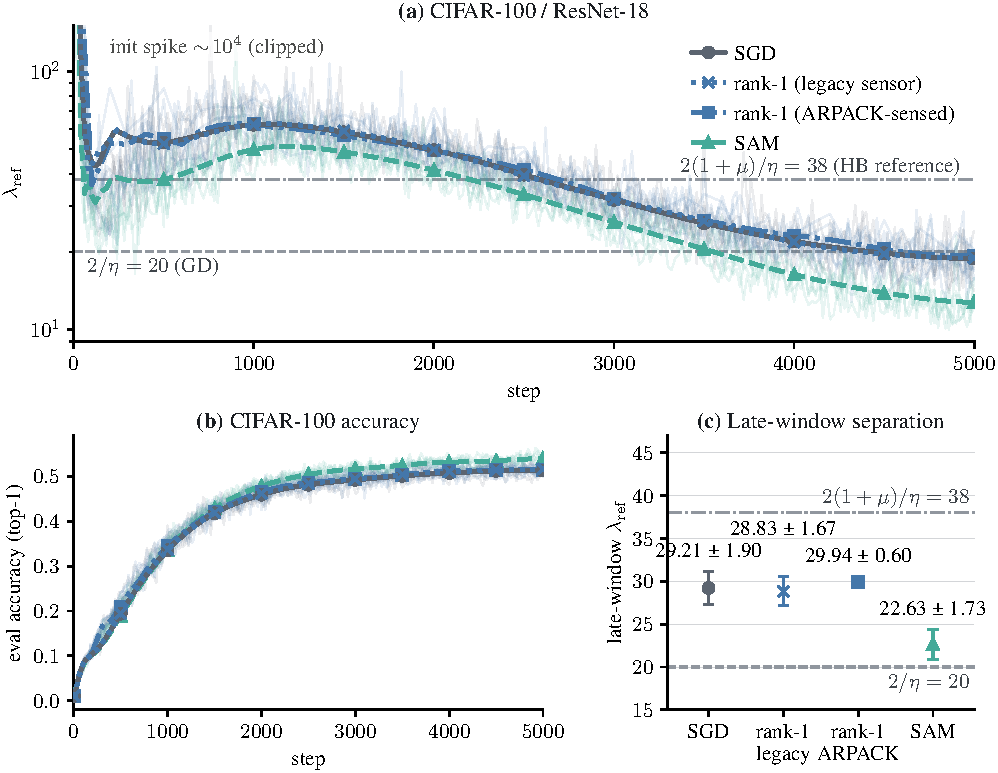
\includegraphics[width=0.95\linewidth]{30_cifar100_r18_control.pdf}
\caption{规模复现：ResNet-18（11.2M）/CIFAR-100，确定性 CUDA，ARPACK 在
确定性 512 样本评估批上测 $\lmax$（$n=5$ 种子）。\textbf{(a)} $\lmax$
轨迹（细线为各 seed、粗线为均值；y 轴截断在 $150$——初始化瞬态
（transient，系统进入稳定模式前的短暂过渡阶段；训练开始时 $\lmax$
冲到 ${\sim}10^{4}$ 的尖峰即瞬态，不代表长期行为）尖到
${\sim}10^{4}$），同时画出 GD 边界 $2/\eta=20$ 与起作用的重球边界
$2(1+\mu)/\eta=38$。\textbf{(b)} 评估精度。\textbf{(c)} 晚窗口（步
$\ge2000$）$\lmax$ 均值 $\pm95\%$ CI：$\{\text{SGD}\approx\text{rank-1}\}$、
SAM 在其下方、CI 不重叠。图中 rank-1 plant 是被钳位的 C3 变体：其自门控
钳位使它在此休眠（触发比例 $\le4\%$，源于下述感知伪收敛，并非体制属性）；
修正后的 ARPACK 感知 plant 以全力开火却仍对尖锐度无影响（有动作仍被钉住，
$n=5$，见 \S\ref{sec:ch08-pinned}）。}
\label{fig:ch08-r18}
\end{figure}

\subsection{方法论插曲：幂迭代伪收敛——proxy 坏了，不是体制坏了}\label{sec:ch08-falseconv}

这一小节是全章最重要的方法论叙事，值得慢慢读。

\textbf{发生了什么。}原版 rank-1 plant 用小批幂迭代估计顶部特征向量，并把
阻尼门控在 $\hat\lambda>2/\eta$ 上。在 ResNet-18 上它读到
$\hat\lambda\approx19<2/\eta=20$，于是只在 $\le4\%$ 的步上触发
（$\approx$SGD）。最初的解读是：“批尖锐度就坐在 $2/\eta$ 上”。

\textbf{ARPACK 直测推翻了这个解读。}在确定性 512 样本批上，顶部特征值其实
是 $\lmax\approx36$（中位 $35.7$、训练全程均值 $40.5$、$88\%$ 的步高于
$2/\eta=20$）。那个 $\approx19$ 是\emph{幂迭代伪收敛}（false
convergence）：两次 HVP 后的早停落在了\emph{次主导瑞利商}上，平均低估
$+45\%$。一句话：\emph{proxy 坏了，不是体制坏了}——随机 EoS 体制本来
好好的，坏的是那个廉价传感器。

这里有一个普适教训，与第~\ref{sec:ch10}~章的“监测器”建议相接：近简并的
重尾谱（近简并 = 前几个特征值几乎相等、“谁是最尖方向”难分伯仲——
此时幂迭代分不清该收敛给谁；重尾 = 除少数极大特征值外、大量方向仍有
可观的曲率；这是 ResNet-18 海森的典型谱形）正是 warm-start 幂迭代最脆弱的环境；当你的
廉价 proxy 读出一个“恰好支持你假设”的数字（“批尖锐度在 $2/\eta$”）时，
这个巧合本身就是值得怀疑的理由。论文的处置是换成确定性批 + ARPACK 直测，
并把测量协议写进结论。

\subsection{true-$\lmax$ plant：执行器真打了，尖锐度不动}\label{sec:ch08-pinned}

\textbf{修好感知。}论文把传感换成 warm-start ARPACK（$k=2$、
$\mathrm{tol}=10^{-2}$），每 $N=20$ 步在同一个确定性批上执行，并去掉原
plant 除数里的 $\max(\cdot,1)$ 下限。于是阻尼除数为
$\lmax/(2/\eta)\approx1.8$，秩-1 阻尼因子每步 $\approx0.44$（即除数蕴含
的瞬时每步因子 $1-1/d$；后文的 $0.46$、$0.39$ 与此同为 $1-1/d$ 的
不同口径——分别由中位除数 $1.86$ 与窗口均值得出，因 $d$ 逐步波动
而略有出入）。

\textbf{预注册（pre-registered，实验前公开承诺合格判据——防止看完
结果再临时改标准、把噪声解读成胜利）合格判据。}主除数判据（中位 $1.86$，门槛 $\ge1.5$）与阻尼
均值判据（每步阻尼的窗口均值实现值 $+0.39$，门槛 $>0.3$）在全部 $n=5$ 个
确定性种子上达标，Ritz 有效力率 $100\%$（以 Ritz 残差判定“传感读数
仍新鲜有效”的步数占比——残差合格说明执行器动用特征向量估计时该估计
未过期，无陈旧性混淆）。辅助的触发率
判据被透明报告：它\emph{没有}在全程 5000 步窗口达标（$83\%$，低于预注册
的 $95\%$），但在实质训练窗口（步 1--4000）内达标（$98.5\%$）。注意
判据的分级：除数与阻尼两条是预注册的\emph{主}判据（成功标准）且已
全部达标；触发率只是``动作在场''的辅助监测而非成功标准，其晚期下滑
有机制解释并被如实披露——不是事后改标准。晚期下探
是``动作起效''而非``动作缺席''：执行器在晚期把 $\lmax$ 拉向目标
$\lambda_{\mathrm{targ}}$，除数\emph{按设计}跌破触发阈值——动作成功的
副作用，不是动作缺席。

\textbf{结局：有动作仍被钉住。}执行器确实在打（除数 $\approx1.8$、每步
阻尼因子 $\approx0.44$），可尖锐度轨迹几乎不动：$\lmax$ 稳态中位数
$[37.2,36.9,39.7,35.6,36.3]$（五个种子）与 vanilla SGD（$33.8\pm3.7$
——此基线为 true-$\lmax$ plant 实验族的伴随 SGD 臂，口径是稳态中位
数的跨种子统计，与表~\ref{tab:ch08-threeway} 的晚期均值口径不同，
故数值有差）重叠。以真实力阻尼\emph{一个}方向钉不住高秩谱：尖锐度在秩-$(n{-}1)$
正交补上重新分布，并且无论阻尼与否都绕当下体制的实际阈值（重球边界
$38$）自稳定。这就是
预测器$\ne$执行器二分的规模版——\emph{有动作仍被钉住}（pinned
despite action）：执行器可验证地全力开火，$\lmax$ 却不出跨种子噪声包络。
它与全批 MLP 体制恰好相反：在那里，同样精确的执行器会上逃逸到
$261.8\pm5.4$（第~\ref{sec:ch09}~章给出两种体制的统一理论视角）。只有
全局动作能降到阈值以下——SAM 同时作用于每个方向。

\subsection{更长日程的外部效度：12000 步 + 标准增强}\label{sec:ch08-long}

5000 步、恒定学习率、无增强是一个欠拟合体制（underfitting regime，模型尚未学满、离峰值精度还远；第~\ref{sec:ch10}~章的局限
(vii)）。为探测排序的外部效度，论文在 12000 步（${\approx}31$ epochs）+
标准 pad/crop + 水平翻转增强下重跑三向（$n=2$ 种子/臂，同一确定性 +
ARPACK 协议）。晚窗口（步 $\ge8000$）$\lmax$：SGD $21.9$、rank-1
$22.8$、SAM $18.1$。三个观察：

\begin{itemize}
  \item SAM 甚至低于 \emph{GD} 边界 $2/\eta=20$；
  \item rank-1 plant 与 SGD 差 ${\sim}1$ 单位（有动作仍被钉住）；
  \item 排序 $\text{SAM}<\{\text{SGD}\approx\text{rank-1}\}$ 不变（逐种子
        差距符号一致，SAM-vs-SGD 为 $-3.4/-4.2$）。
\end{itemize}

SAM 同时拿到最好精度（$0.68$ vs $0.66$）；增强把每一臂都抬高了——作为
参照，5000 步无增强的 CIFAR-100 精度只有 ${\sim}52\%$。

\subsection{ResNet-18 上的 rank-$k$：null 结果，不是第二次机制反驳}\label{sec:ch08-rankk}

rank-$k$ 扫描（$k=1,2,5$，原幂迭代感知 plant）在 ResNet-18 上是平的：
$k=1$：$30.29\pm1.45$、$k=2$：$32.25\pm5.72$、$k=5$：$34.06\pm4.52$
（各 $n=5$）——在该协议下都 $\approx$SGD（ARPACK 测的 $k=1$，即
$28.83\pm1.67$，就是上面三向中的 rank-1；换用 ARPACK 后绝对值有偏移，
$k$-不变结论不变）。此处要分清\emph{两把尺子}：前述``$+45\%$ 低估''
指 plant \emph{内部传感}的两次-HVP 早停止读数（$\hat\lambda\approx19$
vs ARPACK 真值 $\approx36$）；而扫表报告的 $\lmax$ 轨迹来自另一套
结局测量协议——两者不是同一把尺子，故表中幂迭代读数与 ARPACK 只差
约 $1.5$ 单位。

关键在于如何\emph{归因}这个 null：那个 plant 恰恰因 \S\ref{sec:ch08-falseconv}
记录的感知伪收敛而休眠；修正的 true-$\lmax$ $k=1$ plant \emph{确实}开火，
却仍与尖锐度无关（有动作仍被钉住），所以 null 只会\emph{更}成立：任何
$k$ 都没有下逃逸。但论文明确说：这是\emph{控制性}结果，\emph{不是}对“谱
迁移”备择的第二次独立反驳——那次反驳要靠 MLP 多尖锐景观测试（在那里执行
器确实触发、$k$ 确实要紧，见第~\ref{sec:ch09}~章的逐方向结构）。这里只主张
rank-$k$ 的\emph{排序}结论——无 $k$ 下逃逸、唯 SAM——在真实 CNN 上成立。
（``控制性结果''指该实验的作用只是排除“plant 休眠所以测不出”这一干扰
解释、从而加固已有结论，并不提供一条新的独立证据线；独立反驳需要专门
设计的新实验，如 MLP 多尖锐景观测试。）

\subsection{为何 SAM 能而秩-1 不能（实证侧）}\label{sec:ch08-why}

论文 \S5.7 末段给了一个统一的透视：两者的对比不是“局部 vs 全局几何”，而是
\emph{方向性动作 vs 曲率感知动作}作用于同一景观。

SAM 的扰动先把梯度查询点移到
$\theta+\rho\nabla L/\|\nabla L\|$ 再求梯度；一阶展开（Andriushchenko 等人，2022）
显示这给更新加上 $(\rho/\|\nabla L\|)\,H\nabla L$，于是顶部方向被一个
\emph{曲率相关}因子 $1+\rho\lambda_{1}/\|\nabla L\|>1$ 放大——尖锐轴上的
有效步长\emph{变大}，SAM 所追踪的稳定性边界相应\emph{下移}到 $2/\eta$ 之下
（Long 等人，2024）。秩-1 阻尼做的是相反的事：顶部方向被缩到 $1/d<1$，
有效步长变小、边界\emph{上移}到 $y^{*}>0$（形式化见第~\ref{sec:ch09}~章
的命题 1 与两条推论）。两个执行器朝相反方向移动 EoS 阈值；只有曲率放大
型（全方向）的那个到达下逃逸区。

最后校准期望：SAM-vs-其余的分离幅度在 CIFAR-100 三向里 ${\sim}7$ 单位、
在 CIFAR-10 的 X-SAM 设定里 ${\sim}8$、在 MLP 头条里 ${\sim}19$。小批噪声
与动量模糊了分离——所以规模上的复现是\emph{定性}的（排序 + CI 分离），
不是 GD 体制那种精确的 $2/\eta$ 钉住。

\subsection*{本章要点}
\begin{itemize}
  \item 三向对比在 ResNet-18/CIFAR-100（$n=5$、确定性 CUDA + ARPACK）复现
        为\emph{双结局}：$\{\text{SGD}\approx\text{rank-1}\}$ vs SAM
        （$22.63\pm1.73$，CI 不重叠），且多数晚期步低于重球边界 38
        （frac${}<38$：$81\%/82\%/94\%$），与随机 EoS 一致。
  \item 原 plant 的“$\hat\lambda\approx19$、$\le4\%$ 触发”是幂迭代伪
        收敛：ARPACK 直测 $\lmax\approx36$（中位 $35.7$、均值 $40.5$、
        $88\%$ 步 $>20$），$\approx19$ 是落在次主导瑞利商上的 $+45\%$
        低估——proxy 坏了，不是体制坏了。
  \item true-$\lmax$ plant（ARPACK，$k=2$、tol $10^{-2}$、每 $20$ 步、无
        钳位下限）全力开火（除数中位 $1.86$、每步阻尼 $\approx0.44$、
        Ritz 有效力率 $100\%$），$\lmax$ 稳态仍与 SGD 重叠——规模版的
        \emph{有动作仍被钉住}。
  \item 12000 步增强日程保序（SAM $18.1<$ SGD $21.9\approx$ rank-1
        $22.8$；SAM 精度最好 $0.68$ vs $0.66$）；ResNet-18 rank-$k$ 是
        null 而非第二次机制反驳（机制反驳靠 MLP 多尖锐测试）。
  \item SAM 与秩-1 阻尼朝相反方向移动 EoS 阈值：曲率放大因子
        $1+\rho\lambda_1/\|\nabla L\|>1$ 下移边界，$1/d<1$ 上移边界——
        形式化在第~\ref{sec:ch09}~章。
\end{itemize}
